\section{Durchführung}
\label{sec:Durchfuehrung}
In diesem Kapitel werden die einzelnen Schritte des Versuches erklärt.\\

Zunächst wird mittels einer Hall-Sonde die Magnetflussstärke des verwendeten Elektromagneten vermessen, um den Zusammenhang zwischen der Flussstärke und der eingestellten Stromstärke berechnen zu können.\\
Danach wird der Versuch wie in \autoref{fig:vaufbau} aufgebaut.
Das aus der Spektrallampe tretende Licht wird auf ein Geradsichtprisma fokussiert.
Dieses lenkt das Licht wellenlängenabhängig ab.
Ein eingebrachter Polarisationsfilter lässt danach die verschiedenen Übergänge voneinander trennen.
Der Spalt $S_2$ lässt je nach Einstellung nur einen kleinen Wellenlängenbereich, um die zu untersuchende Wellenlänge hindurch.
Zuletzt wird das Licht durch eine Linse auf die Lummer-Gehrcke Platte geleitet und danach mittels einer Kamera photographiert.

\begin{figure}
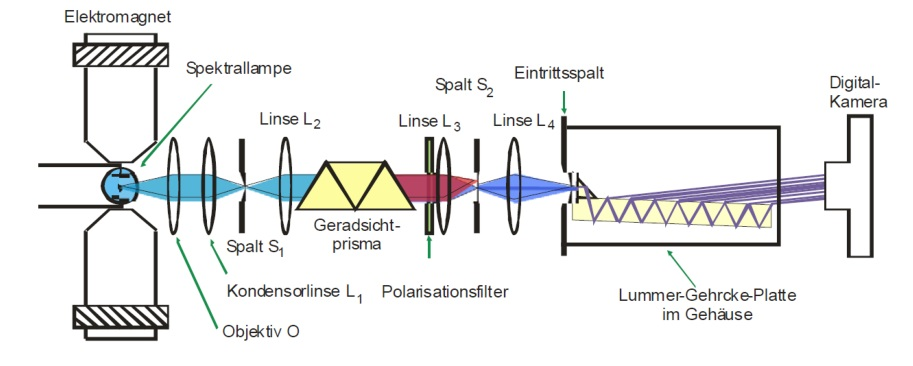
\includegraphics[width=1\textwidth]{content/grafiken/Aufbau.jpg}
\caption{Versuchsaufbau\footnote}
\label{fig:vaufbau}

\end{figure}
\footnotetext{V27 Der Zeemanneffekt, TU Dortmund}

Bei der Justage musste zunächst das Objektiv möglichst nah an die Spektrallampe herangeführt werden, um letztendlich die Intensität des auf die Lummer-Gehrcke Platte einfallenden Strahls zu maximieren.
Der Strahlgang sollte mittig durch alle Linsen führen, um Verluste zu minimieren und in so einem Winkel auf das Eingangsfenster der Lummer-Gehrcke Platte treffen, dass der Strahl in die eigentliche Platte totalreflektiert wird. 
Der Winkel bestimmt auch wo auf der Platte die Linien vorwiegend zu sehen sind und sollte für die Spektrallinie mit 480\,nm möglichst nahe am Eingangsfenster der Platte liegen, da dies ein besseres Bild ergab.
Die Position der Kamera musste auf die Lummer-Gehrcke Platte abgestimmt werden und damit die entstehnden Linien deutlich sichtbar sind, musste der Fokus der Kamera ins Unendliche gelegt, sowie die Belichtungszeit sehr hoch gewählt werden.\\
Untersucht wurde die Aufspaltung der Spektrallinien bei 480\,nm und 643,8\,nm Wellenlänge. Dazu wurde jeweils vier Photos gemacht.
Zwei Photos mit eingeschaltetem Magnetfeld für parallel zum Magnetfeld und senkrecht dazu polarisierte Strahlung und zwei Photos ohne Magnetfeld für dieselben Polarisationen.
